\documentclass{article}
\usepackage{amsmath}
\usepackage{amssymb}
\usepackage{graphicx}
\usepackage{hyperref}
\usepackage[version=4]{mhchem}


\begin{document}
\section*{Problem}
As shown in the figure, \(A B\) is the common chord with the length 32 of two intersecting circles \(O\) and \(O^{\prime}\). The radii are 20 feet and 34 feet, respectively. Find the distance between the centers of the circles.\\
(A) 54\\
(B) 42\\
(C) \(\sqrt{1763}\)\\
(D) 30\\
(E) 40\\
\centering
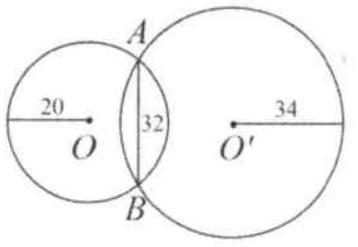
\includegraphics[width=\textwidth]{images/184(1).jpg}

\section*{Solution}
(B).\\
Let the midpoint of the chord \(A B\) be \(P\). Applying the Pythagorean Theorem applied to right triangles \(O P A\) and \(O^{\prime} P A\) gives\\
\(O P^{2}=O A^{2}-A P^{2}=20^{2}-16^{2}=144, \quad O P=12\), And \(O^{\prime} P^{2}=O^{\prime} A^{2}-A P^{2}=34^{2}-16^{2}=900, \quad O^{\prime} P=30\).

The distance between the centers of the circles is \(30+12=\)\\
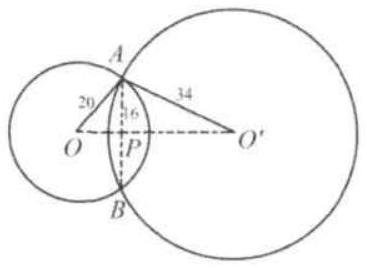
\includegraphics[width=\textwidth]{images/188(1).jpg} 42.

\end{document}
